\documentclass[a4paper]{scrartcl}

%% Language and font encodings
\usepackage[english]{babel}
\usepackage[utf8x]{inputenc}

%% Sets page size and margins
\usepackage[a4paper,top=2cm,bottom=3cm,left=1.9cm,right=1.7cm]{geometry}

%% Useful packages
\usepackage{graphicx}
\usepackage[skip=3pt, format=plain]{caption}
\usepackage{subcaption}

\usepackage{amsmath}

\usepackage{multicol}
\usepackage{matlab-prettifier}
\usepackage{parskip}

\usepackage[colorlinks=true, allcolors=blue]{hyperref}

\renewcommand\thesection{\Alph{section}}

\title{Computational Motor Control - Lab 8}
\subtitle{Walking with Salamandra Robotica - CPG Model}
\author{Florian Kaufmann \and Octave Martin \and Matthias Tsai}

\begin{document}

{\twocolumn

\setlength{\columnsep}{0.5cm}
\maketitle

\section{CPG network implementation}

\subsection*{CPG network layout}
The spinal CPG network of \textit{Salamandra Robotica} is composed of a double chain of oscillators with 10 oscillators each. Each pair of lateral oscillator is assigned to a single joint along the spine and control its angle. The spine joint angle $qs$ is determined by the amplitude $r$ and phase $\theta$ of the associated oscillators as follow:
\begin{subequations}\label{eq:spineCPG}
 \begin{align}
  \theta_{i}^{.} &= 2 \pi f + \sum_{j}\nolimits r_{j} w_{ij} \sin(\theta_{j} - \theta_{i} - \phi_{ij}) \label{eq:spineCPG_phase}\\
  r_{i}^{.} &= a(R_{i}-r_{i}) \label{eq:spineCPG_amplitude}\\
  qs_{i} &= r_{i}(1+\cos(\theta_{i})) - r_{i+10}(1+\cos(\theta_{i+10})) \label{eq:spineCPG_angle}
 \end{align}
\end{subequations}

With $f$ the intrinsic frequency of all the spine oscillators in Hz, $\phi_{ij}$ the nominal phase lag between oscillators $i$ and $j$, $w_{ij}$ the coupling weight between oscillators $i$ and $j$, $a$ the convergence factor set to 1 throughout this report, and $R_{i}$ the nominal spine amplitude.

The limb CPG network is composed of 4 oscillators, each assigned to one limb. The limb joint angle $ql$ is directly controlled by the associated oscillator's phase $\theta$ as follow:
\begin{subequations}\label{eq:limbCPG}
 \begin{align}
  \theta_{i}^{.} &= 2 \pi f_{limb} + \sum_{j}\nolimits r_{j} w_{ij} \sin(\theta_{j} - \theta_{i} - \phi_{ij}) \label{eq:limbCPG_phase}\\
  r_{i}^{.} &= a(R_{limb,i}-r_{i}) \label{eq:limbCPG_amplitude}\\
  ql_{i} &= -\theta_{i} \label{eq:limbCPG_angle}
 \end{align}
\end{subequations}

With $f_{limb}$ the intrinsic frequency of all the limb oscillators in Hz, and $R_{limb,i}$ the nominal limb amplitude.

The code used to implement these equations is available in the appendix \ref{appedix:code_model}.

The final CPG network is composed of a total of 24 oscillators, 20 oscillators controlling the spine joint angles and 4 oscillators controlling the limb joint angles, see Fig.\ref{fig:CPG_layout}. In the next sections we will assign the different coupling strength and phase lag between oscillators for a walking \textit{Salamandra Robotica}.

\begin{figure}
 \centering
 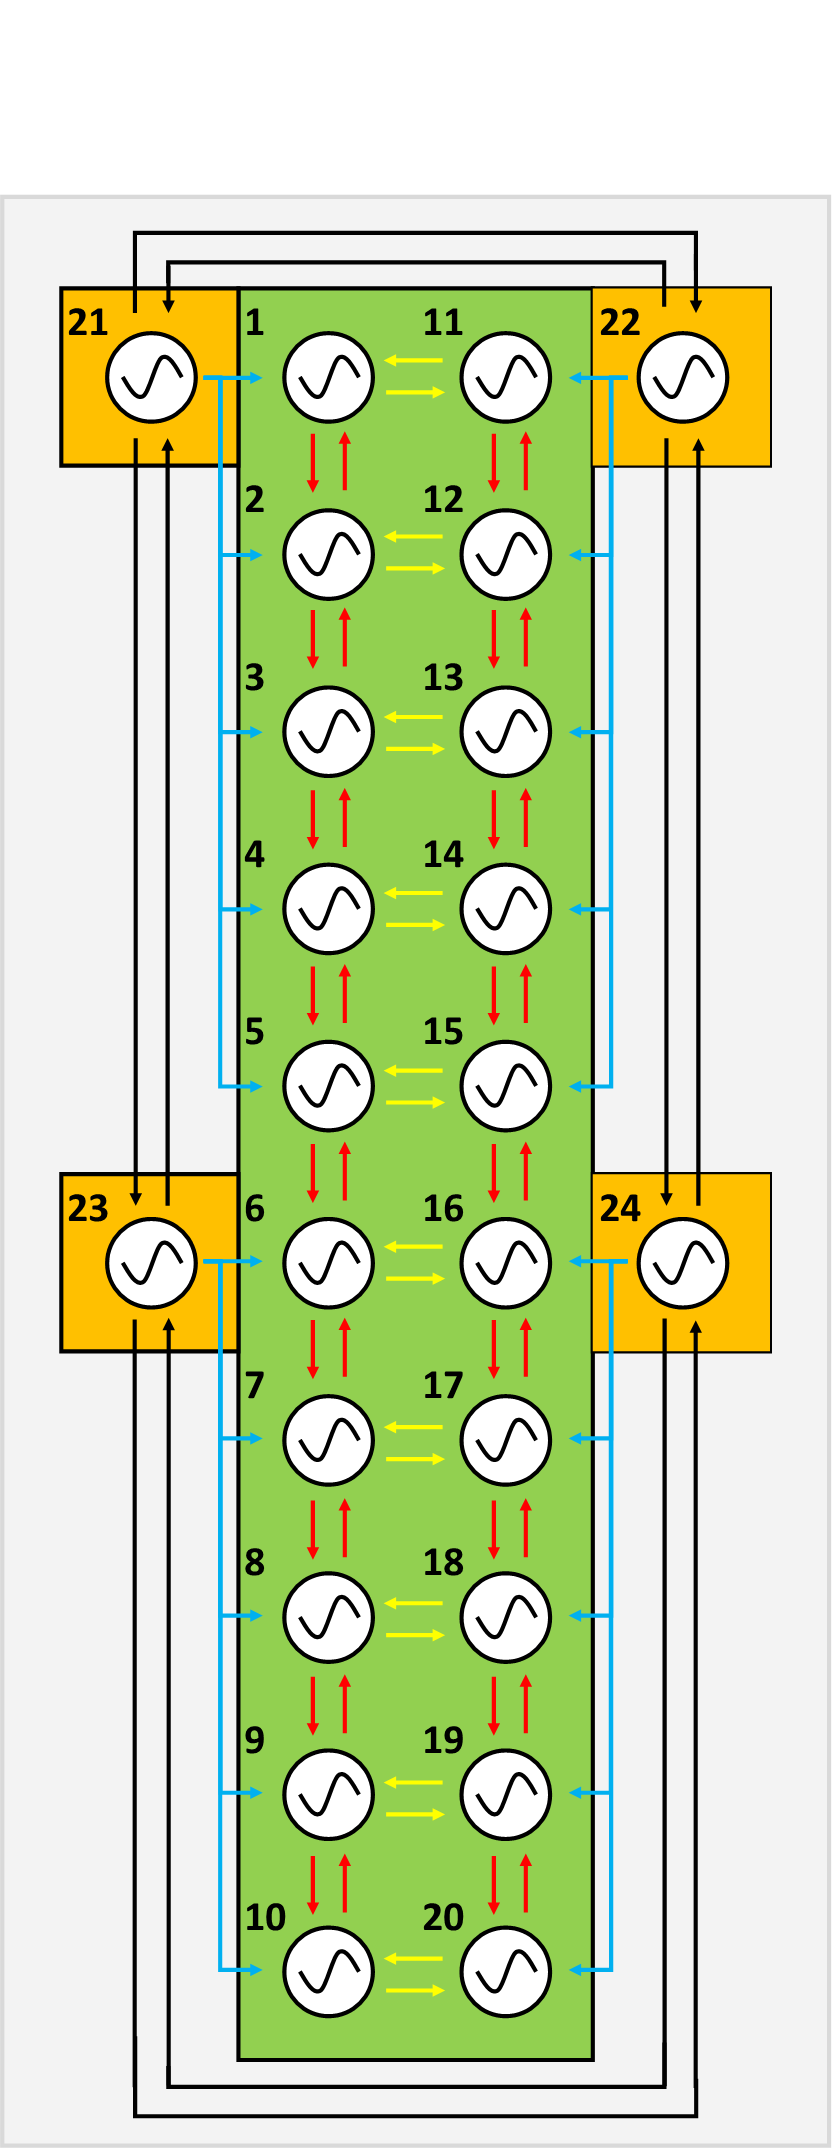
\includegraphics[width=\linewidth]{Figures/CPG_network_V.PNG}
 \caption{\label{fig:CPG_layout} CPG network layout. The area in green correspond to the spinal CPG network with the double chain of oscillators with 10 oscillators each (oscillators 1-10 and 11-20). The area in orange correspond to the limb CPG network (oscillators 21-24). The 4 types of interaction are represented with arrows of different colors: intra-chain in red, inter-chain in yellow, inter-limb in black and limb-spine in blue.}
\end{figure}

\subsection*{Phase lags \& Coupling weights}
There are 4 types of interactions between oscillators in the network: the intra- and inter- chain are interactions between spinal oscillators only, the inter-limb are interactions between limbs oscillators only and limb-spine are interaction between limb and spine oscillators. See Fig.\ref{fig:CPG_layout} and Fig.\ref{fig:weights_lags} for schematic representation of the network's layout, coupling weights and phase lags. 

Intra-chain interaction occurs between successive oscillators in each of the chain of the spinal CPG network. Their nominal phase lags were set to a gradient defined as follow:
\begin{equation}
 \phi_{ij} = \pm \frac{\phi_{total}}{N}
\end{equation}
With $\phi_{total} = 2\pi$ the total phase lag between the first an last oscillator of each axial chain, and $N = 10$ the number of oscillator in the axial chain. The phase lags were defined as positive going from head (\#1 or \#11) to tail (\#10 or \#20) and negative in the opposite direction. The coupling weights were set to $w_{ij} = 10$ for each intra-chain interactions. Both the coupling weights and the phase lags for intra-chain interactions were kept constant throughout this laboratory.

Inter-chain interaction occurs between pair of directly opposite spinal oscillators assigned to a same joint, e.g. oscillators \#1 and \#11. Their nominal phase lags were set to $\phi_{ij} = \pi$, this type of interaction is therefore in anti-phase. The coupling weights were set to $w_{ij} = 10$ for each inter-chain interactions. Both the coupling weights and the phase lags for inter-chain interactions were kept constant throughout this laboratory.

Inter-limb interactions occurs between an oscillator and the oscillator assigned to the limb on the the same side or directly opposite. Their nominal phase lags were set to $\phi_{ij} = \pi$, this type of interaction is therefore in anti-phase. The coupling weights were set to $w_{ij} = 10$ for each inter-limb interactions. Both the coupling weights and the phase lags for inter-limb interactions were kept constant throughout this laboratory.

Contrarily to the other types of interaction, limb-spine interactions are one-sided from limb to spine.  They occurs between a limb oscillator and the spine oscillators on the same sagittal and axial halves. Their nominal phase lags were set to $\phi_{ij} = 0$, this type of interaction is therefore in phase. The coupling weights are higher than for the other types of interaction and were set to $w_{ij} = 30$. While the coupling weights were kept constant throughout the laboratory, the effect of the limb-spine phase lags on the speed was studied by varying this parameter.

\begin{figure}
 \centering
 \begin{subfigure}[b]{\linewidth}
  \centering
  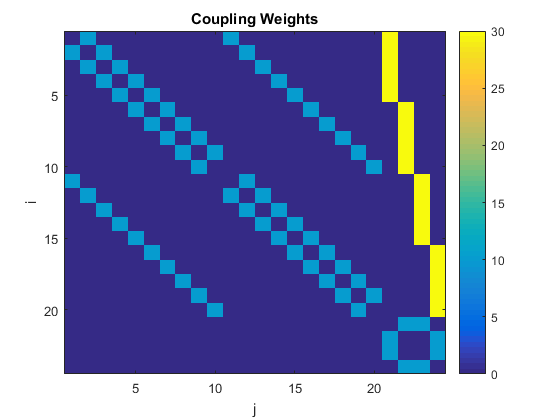
\includegraphics[width=\textwidth]{Figures/weights.png}
  \caption{\label{fig:weights}}
 \end{subfigure}
 \begin{subfigure}[b]{\linewidth}
  \centering
  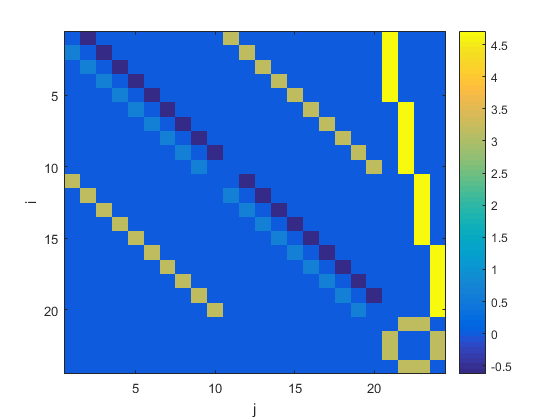
\includegraphics[width=\textwidth]{Figures/phaselags.png}
  \caption{\label{fig:phaselags}}
 \end{subfigure}
 \caption{\label{fig:weights_lags}Coupling weights (\ref{fig:weights}) and phase (\ref{fig:phaselags}) lags between oscillators of the network. The indexing method is the same used in the formulas (\ref{eq:spineCPG}) and (\ref{eq:limbCPG}) with $i$ the current oscillator and $j$ the oscillator interacting with $i$. The two central diagonal correspond to intra-chain interactions, note the discontinuity of the pattern between oscillator \#10 and \#11. The two lateral diagonals correspond to the inter-chain interactions. The circular pattern on the lower right corner correspond to the inter-limb interactions and the pattern above to the limb-spine interactions. The limb-spine phase lag was set to $\phi_{ij} = 3\pi/2$. The representations are not symmetrical with respect to the diagonal because of the one-sided limb-spine interactions.}
\end{figure}

\section{Limb-Spine coordination}

\subsection*{Walking and swimming phase lags comparison}
Before exploring the effect of the limb to spine phase lag $\phi^{limb-spine}$ and spine nominal amplitude $R$ on the walking speed, let's compare the phase lags between walking and swimming conditions. The parameters for each condition are given in the description of Fig.\ref{fig:lags_comp}. 

In walking conditions, we observe two populations of axial oscillators corresponding to the upper and lower halves of the spine, see Fig.\ref{fig:lags_walk}. The phase lags between oscillators of the same population is close to zero. The phase lag between the two populations is stable and the two populations of oscillators are approximatively in anti-phase. This is due to the strong coupling weight between limb oscillators in anti-phase with each others and the corresponding oscillators, see Fig.\ref{fig:CPG_layout}.

In swimming conditions as the contribution of limb-spine interactions is removed, we observe a stable propagating wave along the spinal cord, see Fig.\ref{fig:lags_swim}. The phase lag between successive oscillators going down the spine converges toward the nominal phase lag of $-2\pi/10\approx-0.6$ and the phase lag between the first and last oscillators is a little bit less than $2\pi$.

The behaviour of the spinal oscillators are coherent with the theory and the results from the fifth laboratory.

\begin{figure}
 \centering
 \begin{subfigure}[b]{\linewidth}
  \centering
  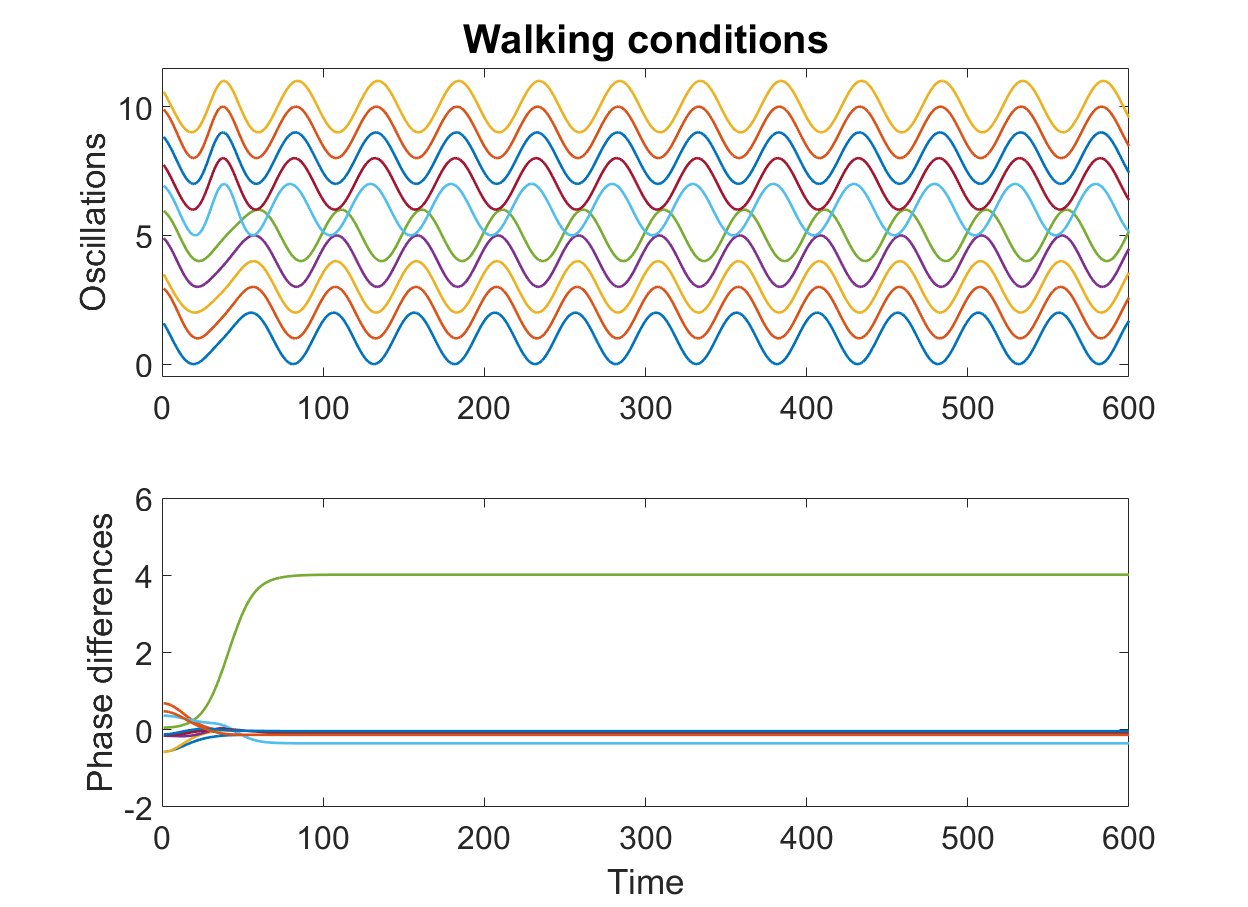
\includegraphics[width=\textwidth]{Figures/figure1A.png}
  \caption{\label{fig:lags_swim}}
 \end{subfigure}
 \begin{subfigure}[b]{\linewidth}
  \centering
  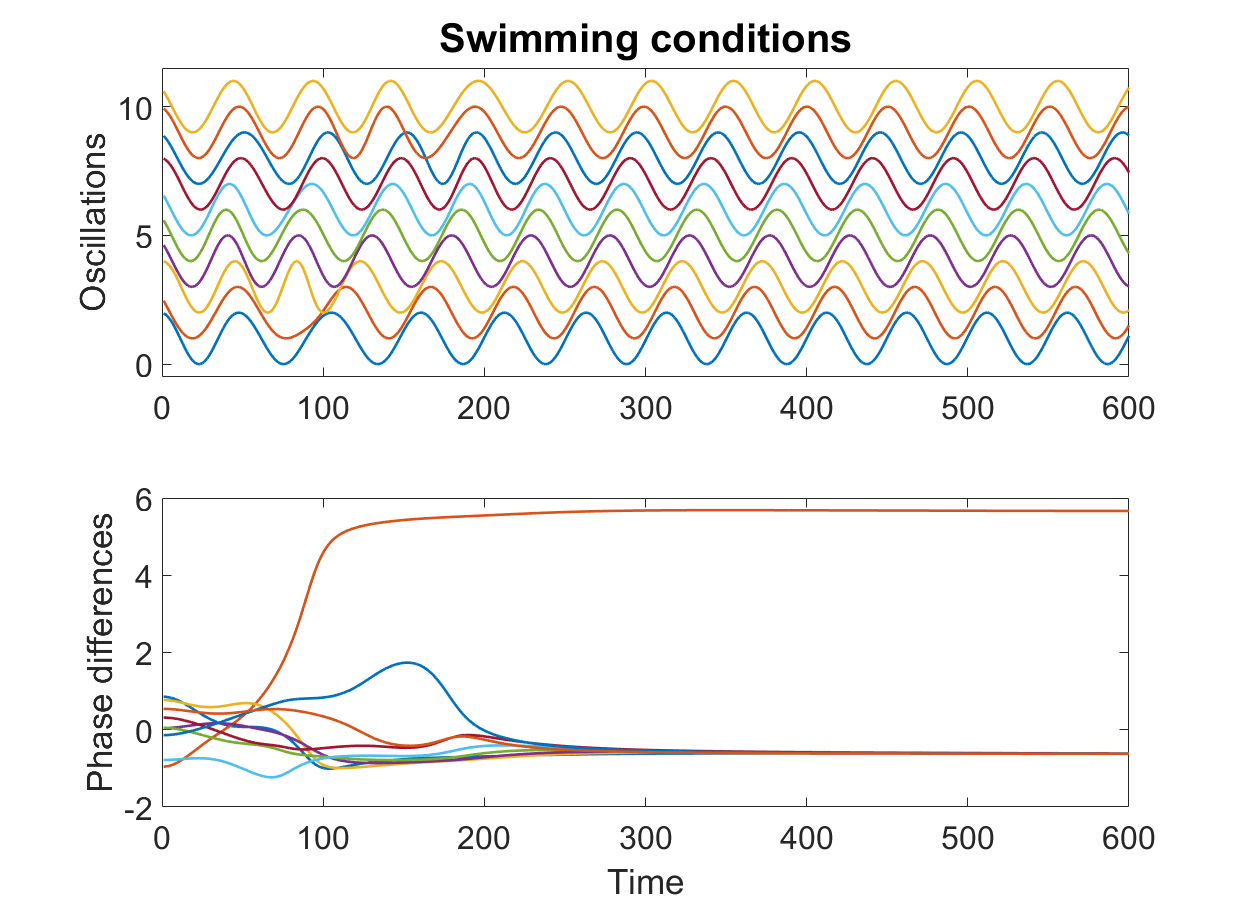
\includegraphics[width=\textwidth]{Figures/figure1B.png}
  \caption{\label{fig:lags_walk}}
 \end{subfigure}
 \caption{\label{fig:lags_comp} Spinal oscillators oscillation and phase difference as a function of time for walking (\ref{fig:lags_walk}) and swimming (\ref{fig:lags_swim}) conditions and for one side only. The parameters in walking conditions were: $f=f_{limb}=1$Hz, $R_{i}=R_{limb,i}=0.3$, $\phi_{ij}^{limb-spine}=0$. For the swimming condition the same parameters were used but the phases of the limb oscillators were set to zero.}
\end{figure}

\subsection*{Influence of limb-spine phase lag on the walking speed}
To measure the walking speed of the salamander we measured the chord length between the points after 3 seconds of simulation and the last point of the simulation, and divided by the elapsed time between the two measurements.

We ran a parameter search on the limb-spine phase offset over 41 linearly equally spaced values between $0$ and $2pi$, and computed for each the walking speed, see Fig.\ref{fig:walking_speed}. The spine nominal amplitude was kept to $R=0.3$. The speed decreases rapidly with increasing phase-limb lag between $0$ and $3pi/5$ with a minimum of $v_{min} = 0.0165$\,m/s for $\phi_{ij}^{limb-spine} = 3\pi/5$. The speed then increases with the limb-spine phase lag between $3\pi/5$ and $3\pi/2$. The maximal walking speed $v_{max} = 0.3907$\,m/s was found for $\phi_{ij}^{limb-spine} = 3\pi/2$. The walking speed then decreases with increasing phase-limb between $3\pi/2$ and $2\pi$. Note that the speeds for $0$ and $2\pi$ phase lags are identical as expected.

We can investigate further the effect of the limb-spine phase lag on velocity by looking at the condition for maximum stride length. \textit{In salamanders, footfalls of diagonal limbs entering stance coincide with the maximal bending of the trunk toward the ipsilateral hindlimb} [\ref{ref:max_stride}]. To quantify the trunk bending we define the total spine bending at a given instant as the sum of the spine joint angle $qs$ at that moment. We will more particularly use the negative trunk bending rate of change. The maximum, minimum and zero crossing of this quantity give respectively the times of maximum bending toward right forelimb, maximum bending toward left forelimb and inter bending straight phase, see Fig.\ref{fig:trunk_bending}. 

The limb implementation is done such that at $ql_{i} = 0$ the limb points downward and is perpendicular to the ground, and at $ql_{i} = \pi/2$ the limb is horizontal and points toward the head of the salamander. For the following we neglect the time delay between the horizontal directed toward the front position of the limb and actual footfall. This assumption seems reasonable given the low height of the salamander. We are looking at the right forelimb specifically and we want to quantify the phase delay between the right forelimb footfall and the maximum trunk bending toward the right forelimb. To do this we used the cross-correlation between the sine of the motor position and the negative trunk bending rate of change and searched for maximum with smallest absolute lag as the two quantities should be in phase to fulfil the maximum stride length condition, see Fig.\ref{fig:corr_ex}. The results are shown in Fig.\ref{fig:corr_speed}. Both curves follow each other closely, and the limb-spine phase lag  for minimum and maximum walking speed correspond exactly to the limb-spine phase lag for minimum and maximum stride length respectively.

\begin{figure}
 \centering
 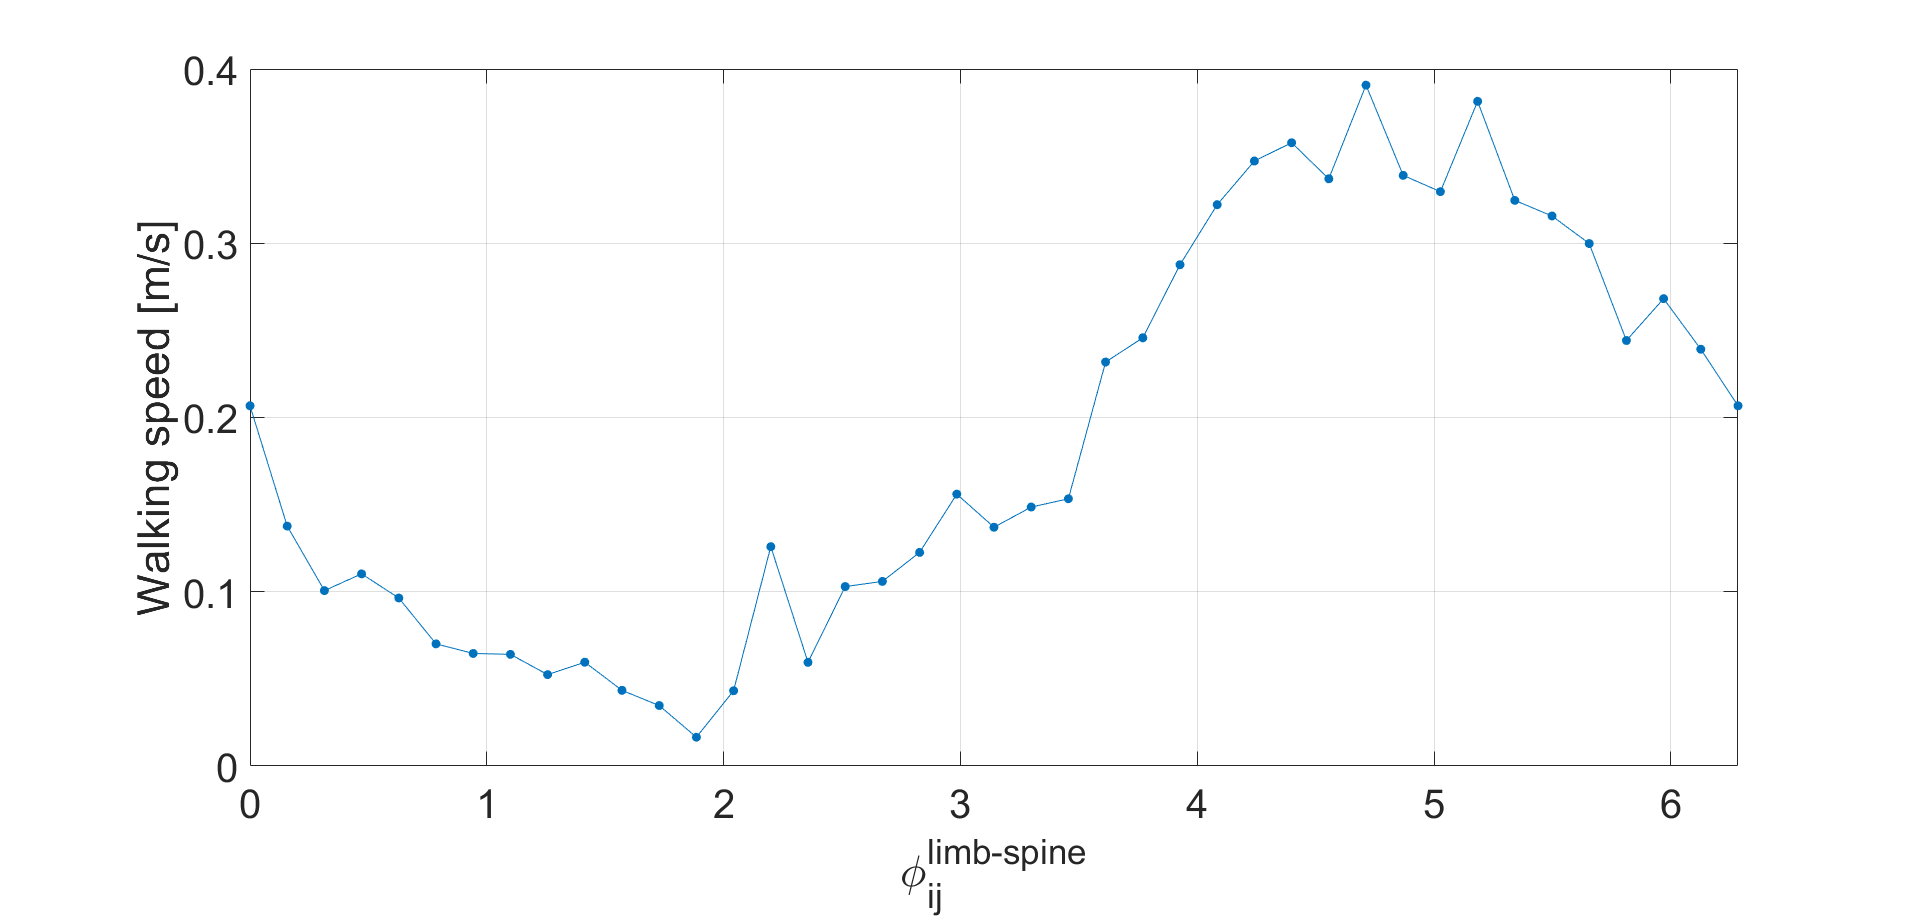
\includegraphics[width=\linewidth]{Figures/figure2A.png}
 \caption{\label{fig:walking_speed} Walking speed versus limb-spine phase offset. 41 linearly equally spaced values between $0$ and $2\pi$ were explored for $\phi_{ij}^{limb-spine}$ The maximal velocity $v_{max} = 0.3907$\,m/s was found for $\phi_{ij}^{limb-spine} = 3\pi/2$.}
\end{figure}

\begin{figure}
 \centering
 \begin{subfigure}[b]{0.45\linewidth}
  \centering
  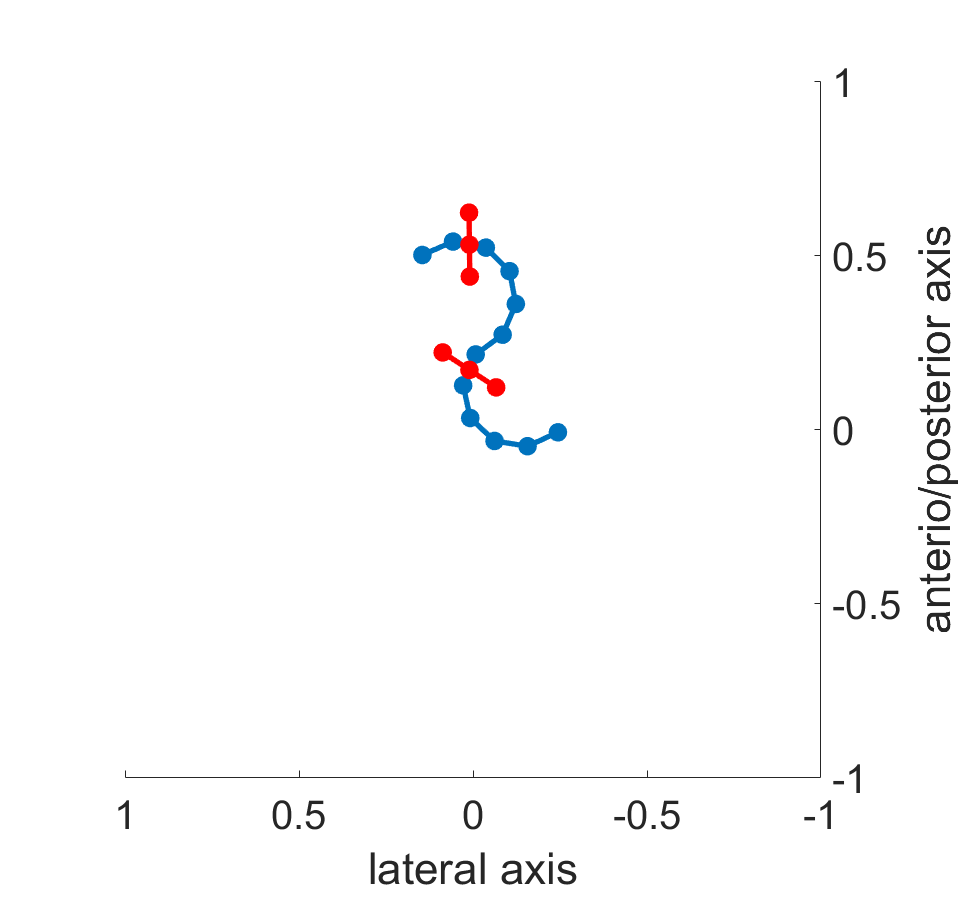
\includegraphics[width=\textwidth]{Figures/figure2Ba.png}
  \caption{\label{fig:right_bend}}
 \end{subfigure}
 \begin{subfigure}[b]{0.45\linewidth}
  \centering
  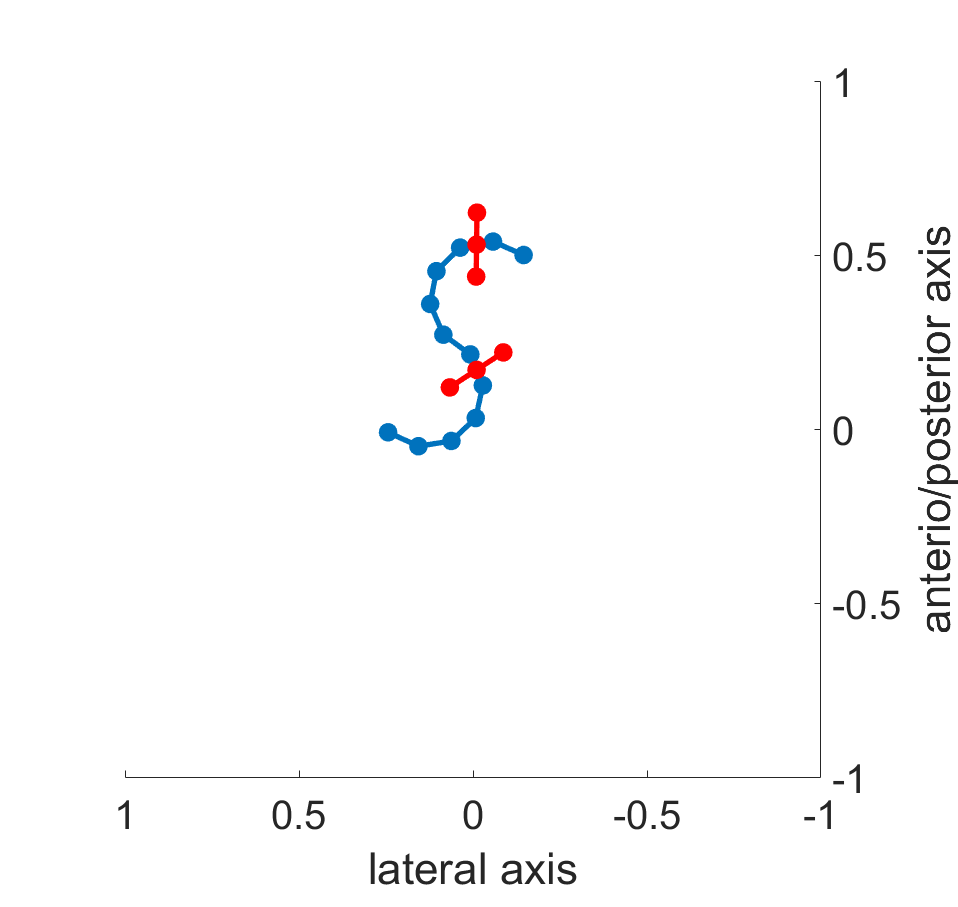
\includegraphics[width=\textwidth]{Figures/figure2Bb.png}
  \caption{\label{fig:left_bend}}
 \end{subfigure}
 \begin{subfigure}[b]{\linewidth}
  \centering
  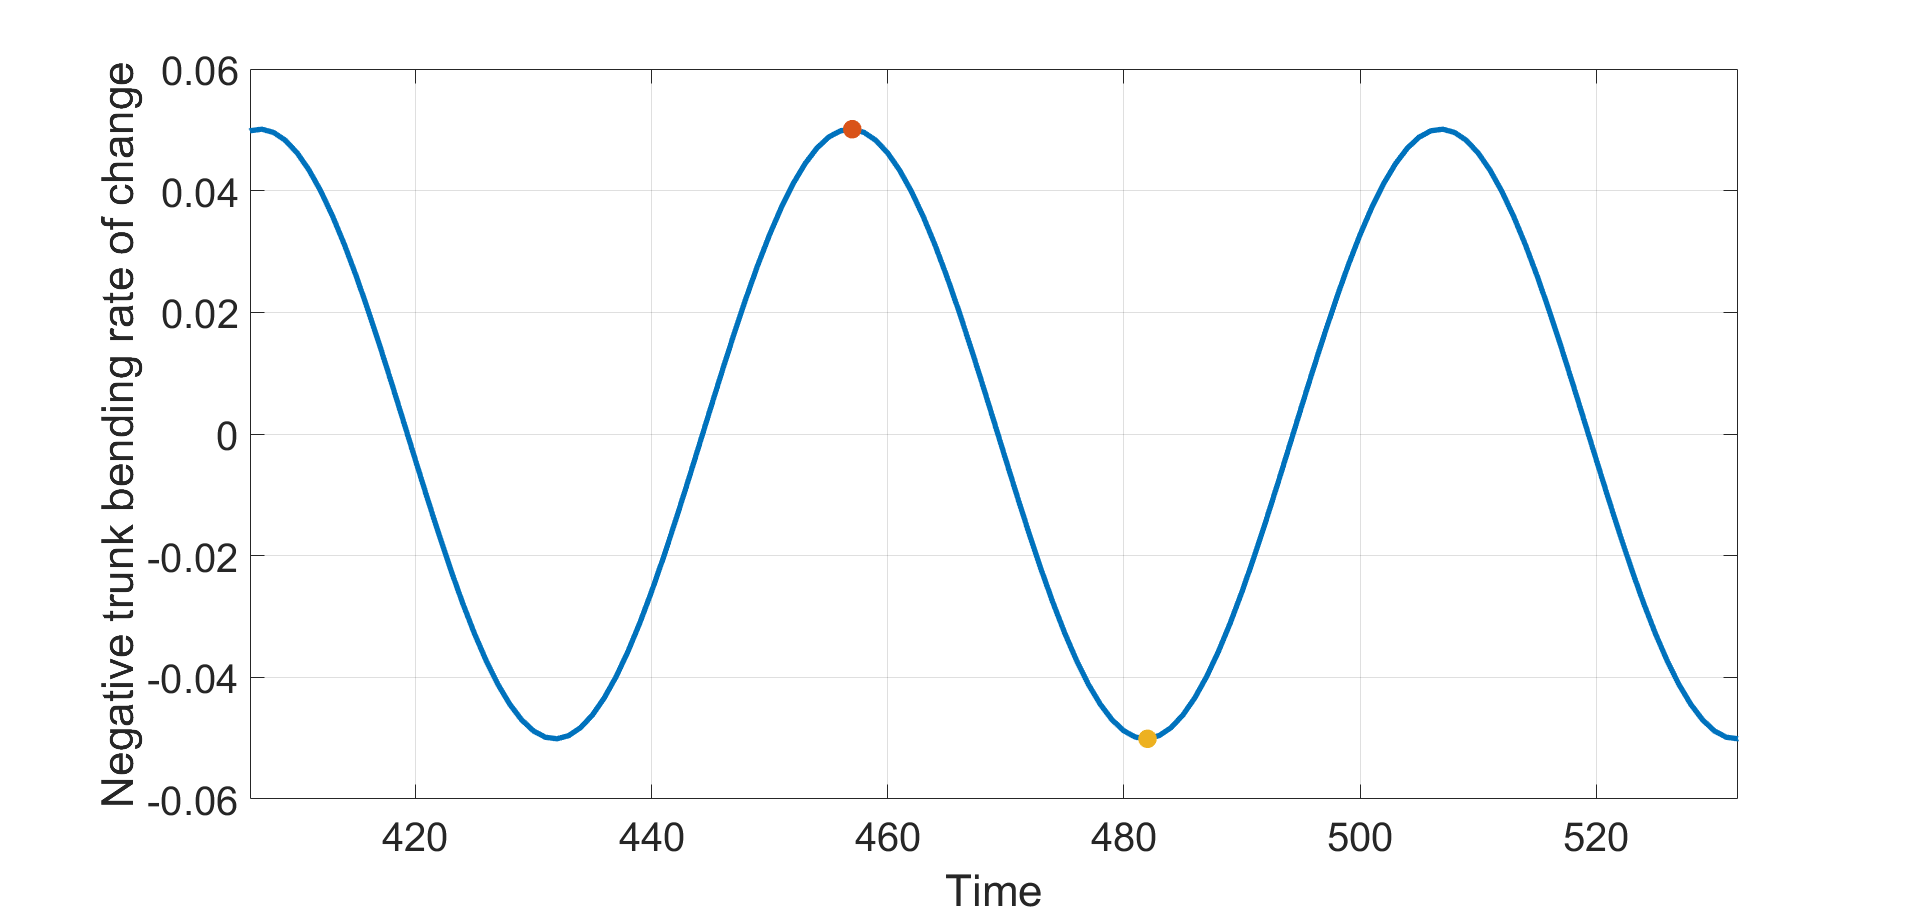
\includegraphics[width=\textwidth]{Figures/figure2Bc.png}
  \caption{\label{fig:rate_bend}}
 \end{subfigure}
 \caption{\label{fig:trunk_bending} Ball-and-stick model of the salamander during maximal trunk bending toward the right forelimb (\ref{fig:right_bend}) and left forelimb (\ref{fig:left_bend}). Time course of the negative trunk bending rate of change (\ref{fig:rate_bend}) with the conditions of the two ball-and-stick model marked by a red point for (\ref{fig:right_bend}) and a yellow point for (\ref{fig:left_bend})}
\end{figure}

\begin{figure}
 \centering
 \begin{subfigure}[b]{\linewidth}
  \centering
  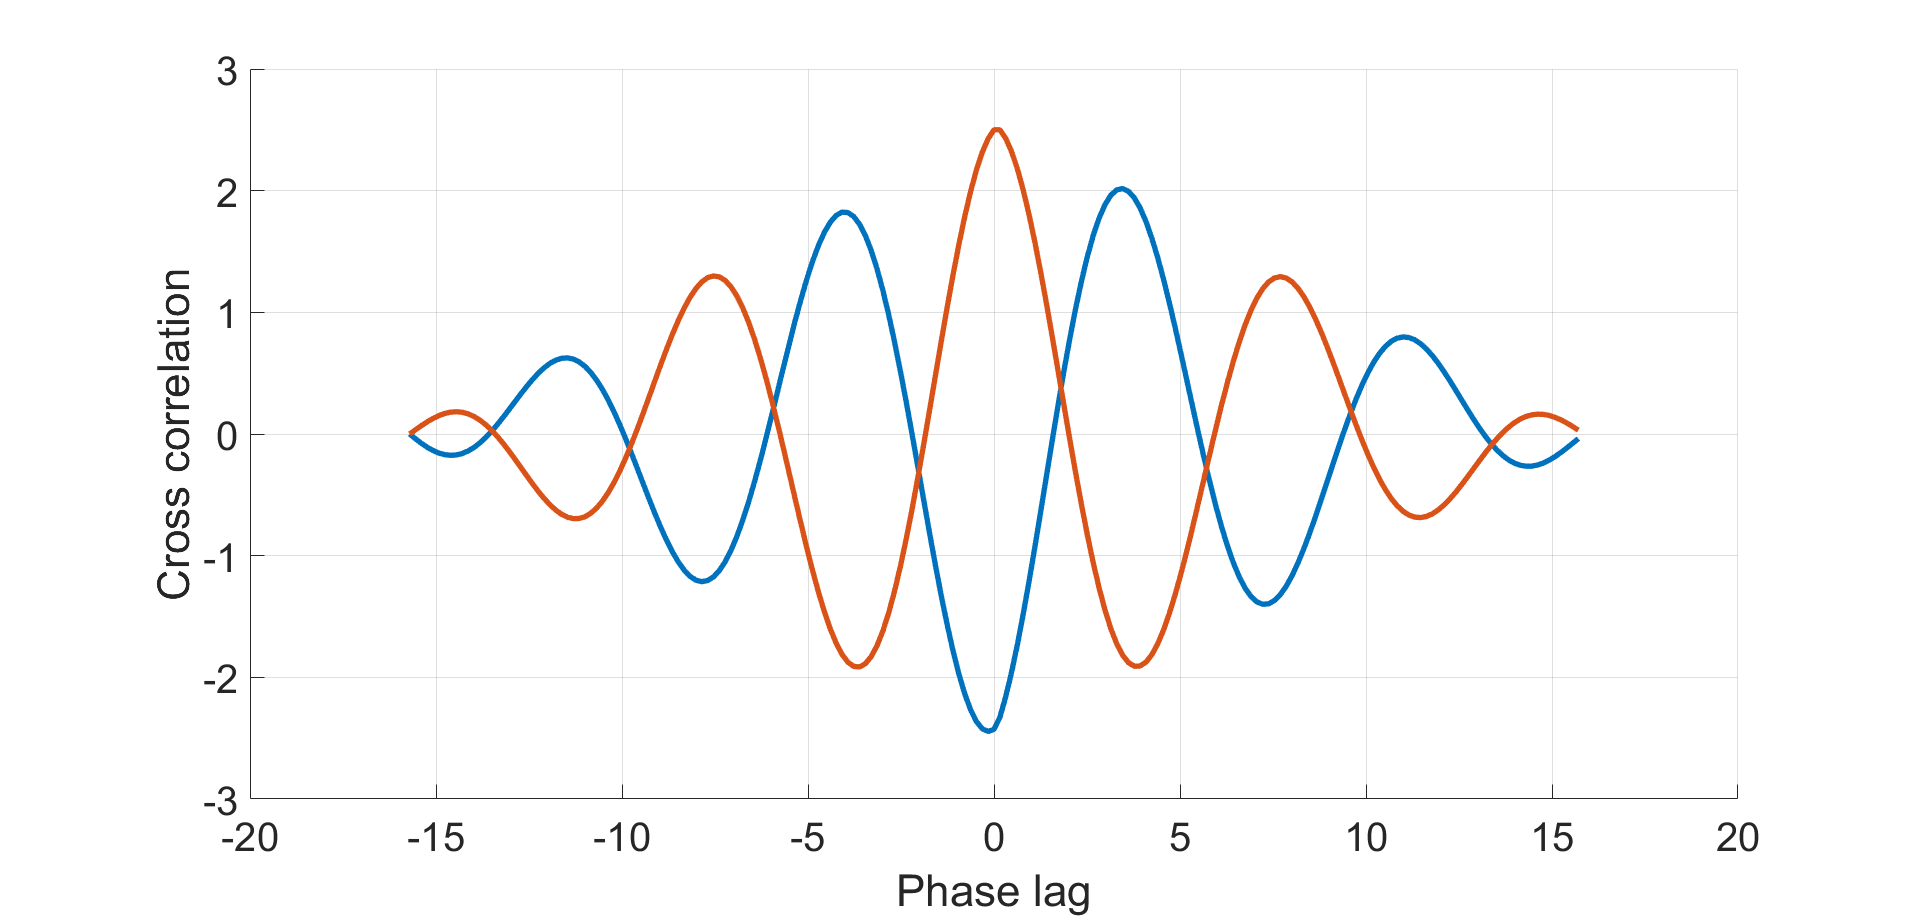
\includegraphics[width=\textwidth]{Figures/figure2Ca.png}
  \caption{\label{fig:corr_ex}}
 \end{subfigure}
 \begin{subfigure}[b]{\linewidth}
  \centering
  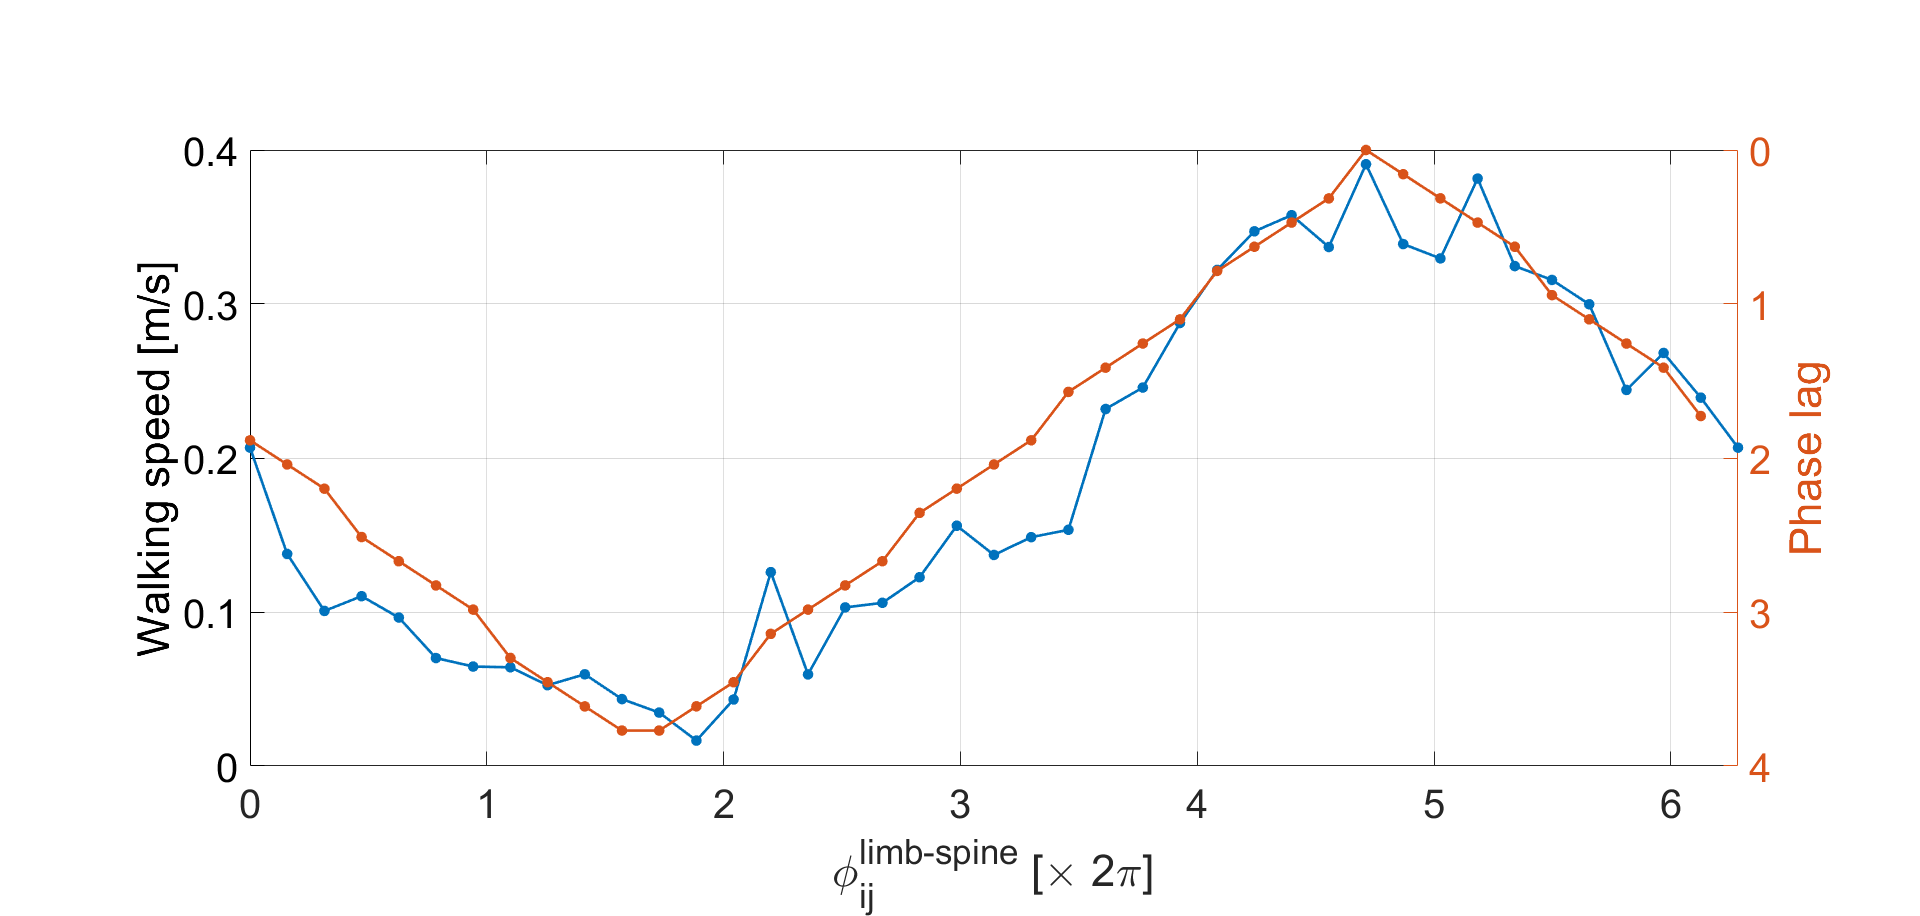
\includegraphics[width=\textwidth]{Figures/figure2Cb.png}
  \caption{\label{fig:corr_speed}}
 \end{subfigure}
 \caption{\label{fig:corr} Cross-correlation between the sine of the motor position and the negative trunk bending rate (\ref{fig:corr_ex}) for $\phi_{ij}^{limb-spine} = 3\pi/5$ in blue and $\phi_{ij}^{limb-spine} = 3\pi/2$ in red. The maximum for the $\phi_{ij}^{limb-spine} = 3\pi/5$ is at approximatively $pi$, the two signal are in anti-phase, this is the opposite of the maximum stride length condition and the speed is minimal. The maximum for the $\phi_{ij}^{limb-spine} = 3\pi/2$ is at $0$, the two signal are in phase, the maximum stride length condition is verified and the speed is maximal. Walking speed and phase lag extracted from cross-correlation (\ref{fig:corr_speed}).}
\end{figure}

\subsection*{Influence of spine nominal amplitude on the walking speed}
In a second time we looked at the influence of the spine nominal amplitude $R$ on the walking speed, see Fig.\ref{fig:walking_speed_R}. The limb-spine phase offset was set to $\phi_{ij}^{limb-spine} = 3\pi/2$. We ran a parameter search on the spine nominal amplitude $R$ over 56 linearly equally spaced values between $0$ and $0.55$, and computed for each the walking speed. $R = 0.55$ is close to the maximal value of $R$ which yields to the maximal physically realisable hinge joint angle.

First the walking speed increases slowly with the spine nominal amplitude between $R=0$ and $R=0.25$ with speed going from $v = 0.2$\,m/s to $v = 0.3$\,m/s. Then the speed rapidly increases with the increasing amplitude between $0.25$ and $0.37$ where the speed reaches $v = 0.5322$\,m/s. The walking speed then reaches a plateau for $R=0.37$ and only increases slowly.

With $R=0$, i.e. no body bend, the stride length is fully determined by the limb length. During walking, higher trunk bending yield to higher stride length and therefore increases the walking speed. 
 
\begin{figure}
 \centering
 \begin{subfigure}[b]{0.45\linewidth}
  \centering
  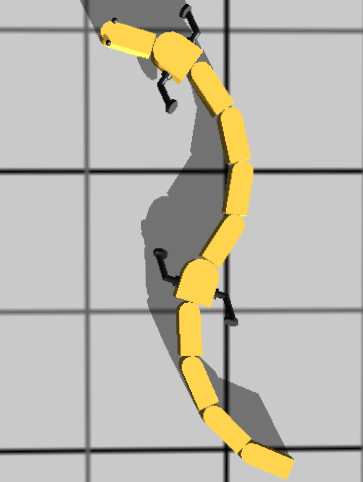
\includegraphics[width=\textwidth]{Figures/figure3Ab.png}
  \caption{\label{fig:bend_R_0.25}}
 \end{subfigure}
 \begin{subfigure}[b]{0.45\linewidth}
  \centering
  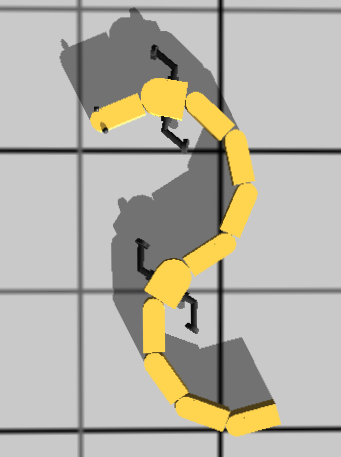
\includegraphics[width=\textwidth]{Figures/figure3Ac.png}
  \caption{\label{fig:bend_R_0.37}}
 \end{subfigure}
 \begin{subfigure}[b]{\linewidth}
  \centering
  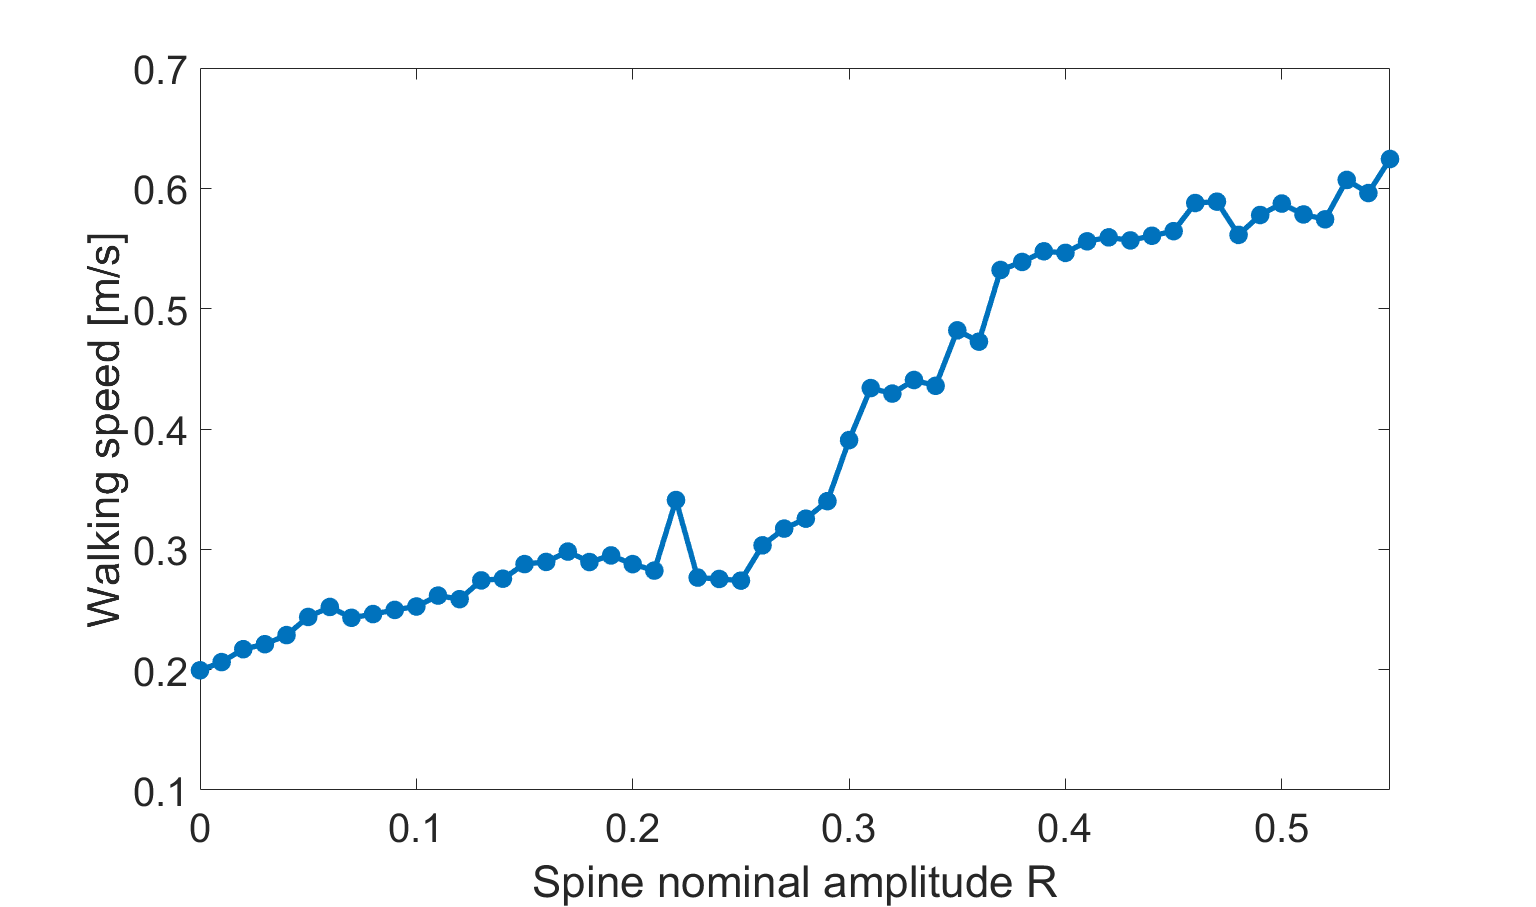
\includegraphics[width=\linewidth]{Figures/figure3Aa.png}
  \caption{\label{fig:speed_R}}
 \end{subfigure}
 \caption{\label{fig:walking_speed_R} Walking speed versus spine nominal amplitude $R$ (\ref{fig:speed_R}). 56 linearly equally spaces values between $0$ and $0.55$ were explored. The walking speed increases with the nominal amplitude and reaches a plateau for $R=0.37$. Maximal body bend for $R=0.25$ (\ref{fig:bend_R_0.25}) and $R=0.37$ (\ref{fig:bend_R_0.37}).}
\end{figure}

\section{Land-to-water transitions}
In this part we will study the land-to-water transition. To switch between walking and swimming the intrinsic frequencies $f$ and $f_{limb}$ as well as the nominal amplitudes $R$ and $R_{limb}$ were made to depend on the x coordinate of the salamander GPS.

Two lines parallel to the land-to-water transition line were defined, one passing through $(x_{switch},0,0)$ and another passing through $(x_{swim},0,0)$. For position with x coordinate bellow $x_{switch}=0.175$\,m the salamander is in walking mode. For position with x coordinate above $x_{swim}=0.575$\,m the salamander is in swimming mode. In between the salamander is in a transition mode.

In walking mode the intrinsic frequencies were fixed to $f=1$\,Hz and $f_{limb}=1$\,Hz. The nominal amplitude were set to $R=0.37$\,m and $R_{limb}=0.3$\,m.

In swimming mode the intrinsic frequencies were fixed to $f=1.5$\,Hz and $f_{limb}=0$\,Hz. The nominal amplitude were set to $R=0.42$\,m and $R_{limb}=0$\,m. The limb angle also fixed to $q_{limb}=-\pi/2$. 

During the transition phase the parameters target values are determined using the transition function shown in Fig.\ref{fig:saturation}. For each parameter the actual parameter value is determined by the mean of the target and the current values with weights of 1 and 10 respectively. This was done to smoothen the variation of the values. Indeed the GPS x-coordinate is given for the salamander head which yield to not monotonically increasing x-coordinates causing fast variations of the parameters values with relatively large amplitudes.

Going from walking to swimming mode both the spine intrinsic frequency and nominal amplitude increases from their walking mode values to their swimming mode values (see the values above). The limb nominal amplitude stay constant during the transition then drops to its swimming value $R_{limb}=0$\,m. The limb intrinsic frequency increases to $f_{limb,max}=1.2$\,Hz before dropping to its swimming value $R_{limb}=0$\,m. Setting the limb intrinsic frequency and nominal amplitude to zero in swimming mode free the spine oscillators from the large limb-spine coupling in walking mode, enabling them to respect the commanded phase lag along the spine.

\begin{figure}
	\centering
	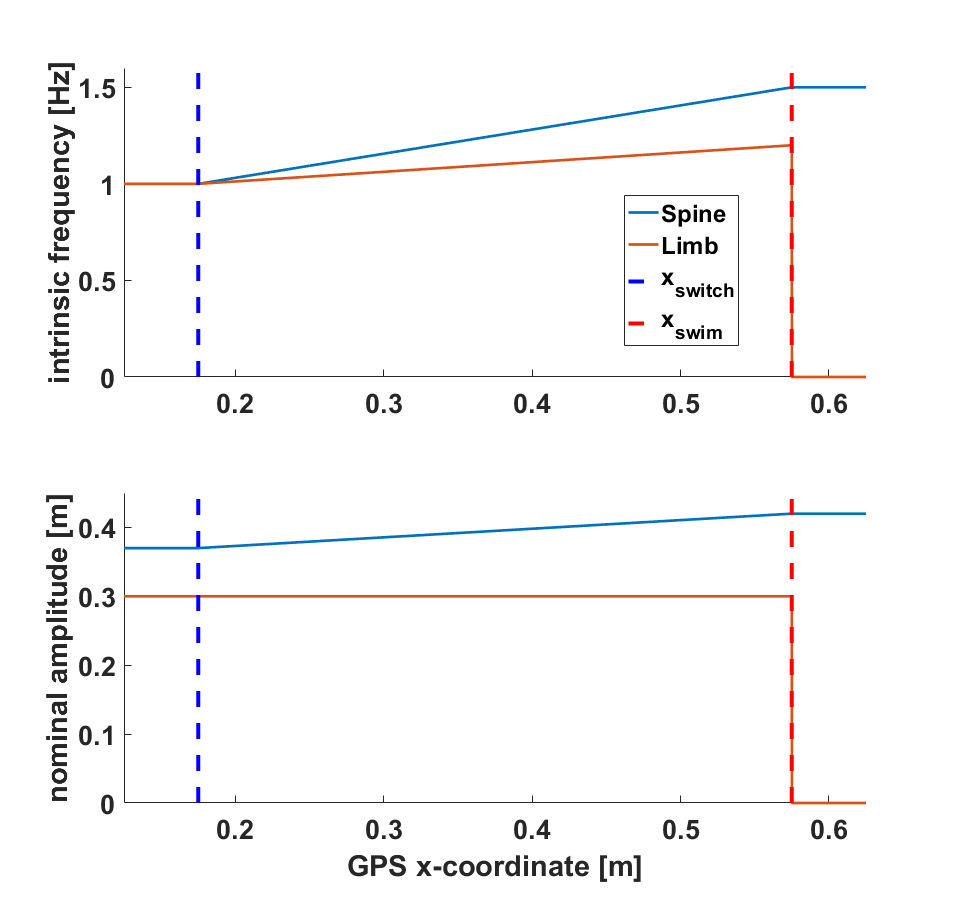
\includegraphics[width=\linewidth]{Figures/saturation.png}
	\caption{\label{fig:saturation}Spine and limb intrinsic frequencies (top) and nominal amplitudes (bottom) determined by the saturation function depending on the GPS x-coordinate. $x_{switch}$ and $x_{swim}$ are shown with blue and red dotted lines respectively.}
\end{figure}

The limb and spine angles along with the GPS-x coordinates are plotted as a function of time in Fig.\ref{fig:land_to_water}. During walking, the characteristic phase opposition between upper and lower halves oscillators can be seen as well as the phase opposition of the limbs. During swimming the travelling wave can been seen from the shifted wave fronts along the spine. The limb angles are fixed during swimming. The transition between walking and swimming modes is relatively smooth and doesn't stall the salamander too much.

\begin{figure}
	\centering
	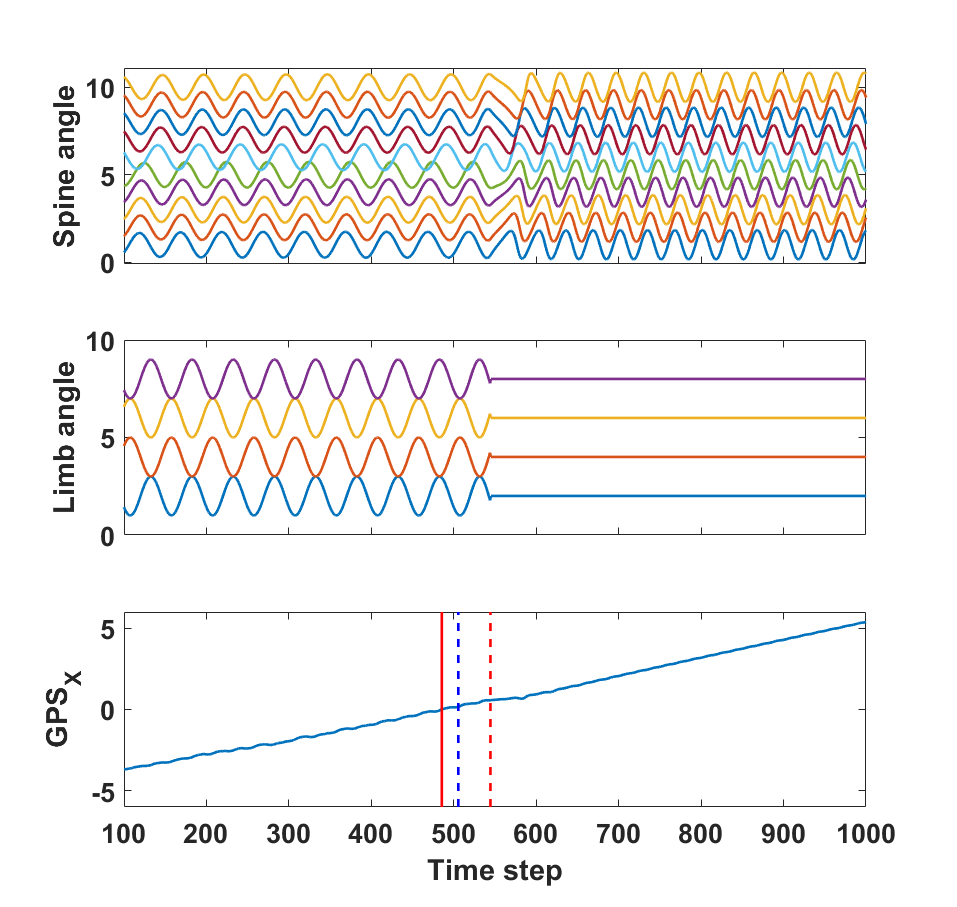
\includegraphics[width=\linewidth]{Figures/land_water_angles.png}
	\caption{\label{fig:land_to_water}Spine and limb angles as well as GPS x-coordinate as a function of time during land-to-water transition. The times for zero-, $x_{switch}$- and $x_{swim}$- crossing are marked with plain red line, dotted blue line and dotted red line respectively.}
\end{figure} 

A video of the simulation is available on this \href{https://drive.switch.ch/index.php/s/9Rfjdp8Z16rn1Pc}{SwitchDrive} and the code for the the function \textit{limbCPGsaturation} is available in the appendix \ref{appedix:code_saturation}. 

\section{Water-to-land transitions}
In this part we study the water-to-land transition. We used the same implementation and same parameters values as for the land-to-water transition.

The angles and x-coordinates are shown in Fig.\ref{fig:water_to_land} and a video of the simulation is available on this \href{https://drive.switch.ch/index.php/s/9Rfjdp8Z16rn1Pc}{SwitchDrive}. Here again the transition is smooth.

\begin{figure}
	\centering
	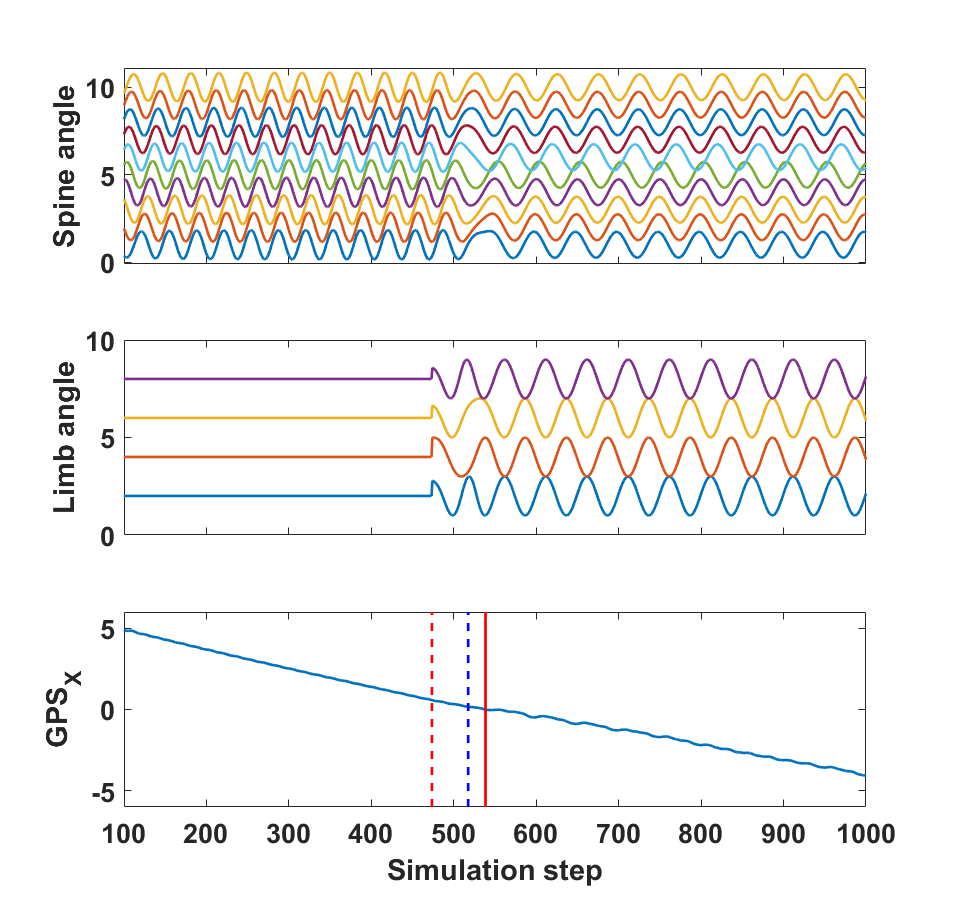
\includegraphics[width=\linewidth]{Figures/water_land_angles.png}
	\caption{\label{fig:water_to_land}Spine and limb angles as well as GPS x-coordinate as a function of time during water-to-land transition. The times for zero-, $x_{switch}$- and $x_{swim}$- crossing are marked with plain red line, dotted blue line and dotted red line respectively.}
\end{figure} 


\begin{thebibliography}{9}

\bibitem{c1} Konstantinos Karakasiliotis, Nadja Schilling, Jean-Marie Cabelguen, Auke Jan Ijspeert, \textit{Where are we in understanding salamander locomotion: biological and robotic perspectives on kinematics}, Biological Cybernetics, 2012,  \label{ref:max_stride}

\end{thebibliography}

%-------------------------------------------------------------------------------------------------

{\onecolumn
\appendix
\section{Implementation code for CPG network}\label{appedix:code_model}
The following code correspond to the implementation of the equations (\ref{eq:spineCPG_phase}) and (\ref{eq:limbCPG_phase}):
\begin{lstlisting}[style=Matlab-editor,basicstyle=\mlttfamily,numbers=none]
dtheta = 2*pi*[f*ones(20,1);f_limb*ones(4,1)] + ...
sum(repmat(r',24,1).*w.*sin(repmat(theta,1,24)'-repmat(theta,1,24)-phi),2);
\end{lstlisting} 

The following code correspond to the implementation of the equations (\ref{eq:spineCPG_amplitude}) and (\ref{eq:limbCPG_amplitude}):
\begin{lstlisting}[style=Matlab-editor,basicstyle=\mlttfamily,numbers=none]
a = 1;  % convergence coefficient not provided in the template
dr = a*([R*ones(20,1);R_limb*ones(4,1)]-r);
\end{lstlisting} 

The following code correspond to the implementation of the equation (\ref{eq:spineCPG_angle}):
\begin{lstlisting}[style=Matlab-editor,basicstyle=\mlttfamily,numbers=none]
qs = r(1:10).*(1+cos(theta(1:10)))-r(11:20).*(1+cos(theta(11:20)));
\end{lstlisting} 

The following code correspond to the implementation of the equation (\ref{eq:limbCPG_angle}):
\begin{lstlisting}[style=Matlab-editor,basicstyle=\mlttfamily,numbers=none]
qlimb = -theta(21:24);	% - to resolve wrong limbs rotation direction 
\end{lstlisting} 

\section{Implementation code for saturation function}\label{appedix:code_saturation}
\begin{lstlisting}[style=Matlab-editor,basicstyle=\mlttfamily,numbers=none]
function [f_out, f_limb_out, R_out, R_limb_out, is_swimming]=limbCPGsaturation(f, f_limb, R, R_limb, gps)

    persistent is_init...
               is_wimming...
               x_swim   x_switch ...
               f_spine_walk f_spine_swim...
               R_spine_walk R_spine_swim...
               f_limb_walk  f_limb_swim f_limb_max...
               R_limb_walk  R_limb_swim R_limb_max;
           
    if isempty(is_init)
        is_init=true;
        
        if gps > x_swim
            is_swimming = true;
        else
            is_swimming = false;
        end
        
        x_swim = 0.575;
        x_switch = 0.175;
        
        f_spine_walk = 1;
        f_spine_swim = 1.5;
        
        R_spine_walk = 0.37;
        R_spine_swim = 0.42;
        
        f_limb_walk = 1;
        f_limb_swim = 0;
        f_limb_max = 1.2;
        
        R_limb_walk = 0.3;
        R_limb_swim = 0;
        R_limb_max = 0.3;
        
    end
    
    if gps > x_swim
        is_swimming=true;
        
        f_out = f_spine_swim;
        f_limb_out = f_limb_swim;
        R_out = R_spine_swim;
        R_limb_out = R_limb_swim;
        
    elseif gps < x_switch
        is_swimming=false;
        
        f_out = f_spine_walk;
        f_limb_out = f_limb_walk;
        R_out = R_spine_walk;
        R_limb_out = R_limb_walk;
        
    else
        is_swimming=false;
        
        Dx = x_swim-x_switch;
        dx = gps-x_switch;
        
        f_out = f_spine_walk + dx*(f_spine_swim-f_spine_walk)/Dx;
        f_limb_out = f_limb_walk + dx*(f_limb_max-f_limb_walk)/Dx;
        R_out = R_spine_walk + dx*(R_spine_swim-R_spine_walk)/Dx;
        R_limb_out = R_limb_walk + dx*(R_limb_max-R_limb_walk)/Dx;
        
        f_out = (10*f + f_out)/11;
        f_limb_out = (10*f_limb + f_limb_out)/11;
        R_out = (10*R + R_out)/11;
        R_limb_out = (10*R_limb + R_limb_out)/11;
        
    end

end
\end{lstlisting} 
\end{document}